\chapter[Introduction]{Introduction} \label{ch:introduction}

The fundamental link between transportation and urban form creates a feedback relationship between land development, travel needs, viability of alternative modes, accessibility, and other important characteristics of the urban transportation system.
Numerous "top-down" and "bottom-up" models have been designed to analyze and forecast the behaviour of urban regions and interaction of their transportation and land use systems.
Since urban systems are complex in nature and require "re-solving" over and over, data science process models present a good fit for this task with their iterative structure.

Increased digitization of human activity, such as introduction of the POLARIS land registration system by the Government of Ontario in 1985, produces a wealth of new information that can be used to study interactions between land use and transportation at a fine spatial and temporal scale.
Teranet's dataset of real estate transactions presents a wealth of information on the housing market of Ontario and can be used for empirical studies of transportation-land use interaction.
However, along with the opportunities, the new data sources also present new challenges.
Teranet's dataset has some data quality issues that need to be addressed and might require special skills to work with due to its size.
But most importantly, it is very limited in the number of features available for each transaction.

One of the major challenges of working with Teranet's data is the lack of features describing each transaction, namely the type of property being sold.
As Teranet's records have timestamps (dates) and coordinates of parcel centroids for each record, they can be joined with other data sources via temporal and spatial relationships, integrity of which needs to be maintained when combining data sources to ensure semantic interoperability.
These relationships are implemented through a standardized data preparation workflow using Python via a series of jupyter notebook which was designed as a part of this master's thesis.
In addition, since all the available sources of land use information have their limitations, a prototype of a machine learning workflow to classify land use from the housing market dynamics is proposed and tested within this thesis.

This thesis generally follows the structure proposed by CRISP-DM, a comprehensive data mining methodology and a process model\cite{Shearer2000} (shown on figure~\ref{fig:crisp_dm}).
CRISP-DM breaks down the life cycle of a data mining project into six phases: business understanding, data understanding, data preparation, modeling, evaluation, and deployment.

\begin{figure}[hbt!]
    \centering
    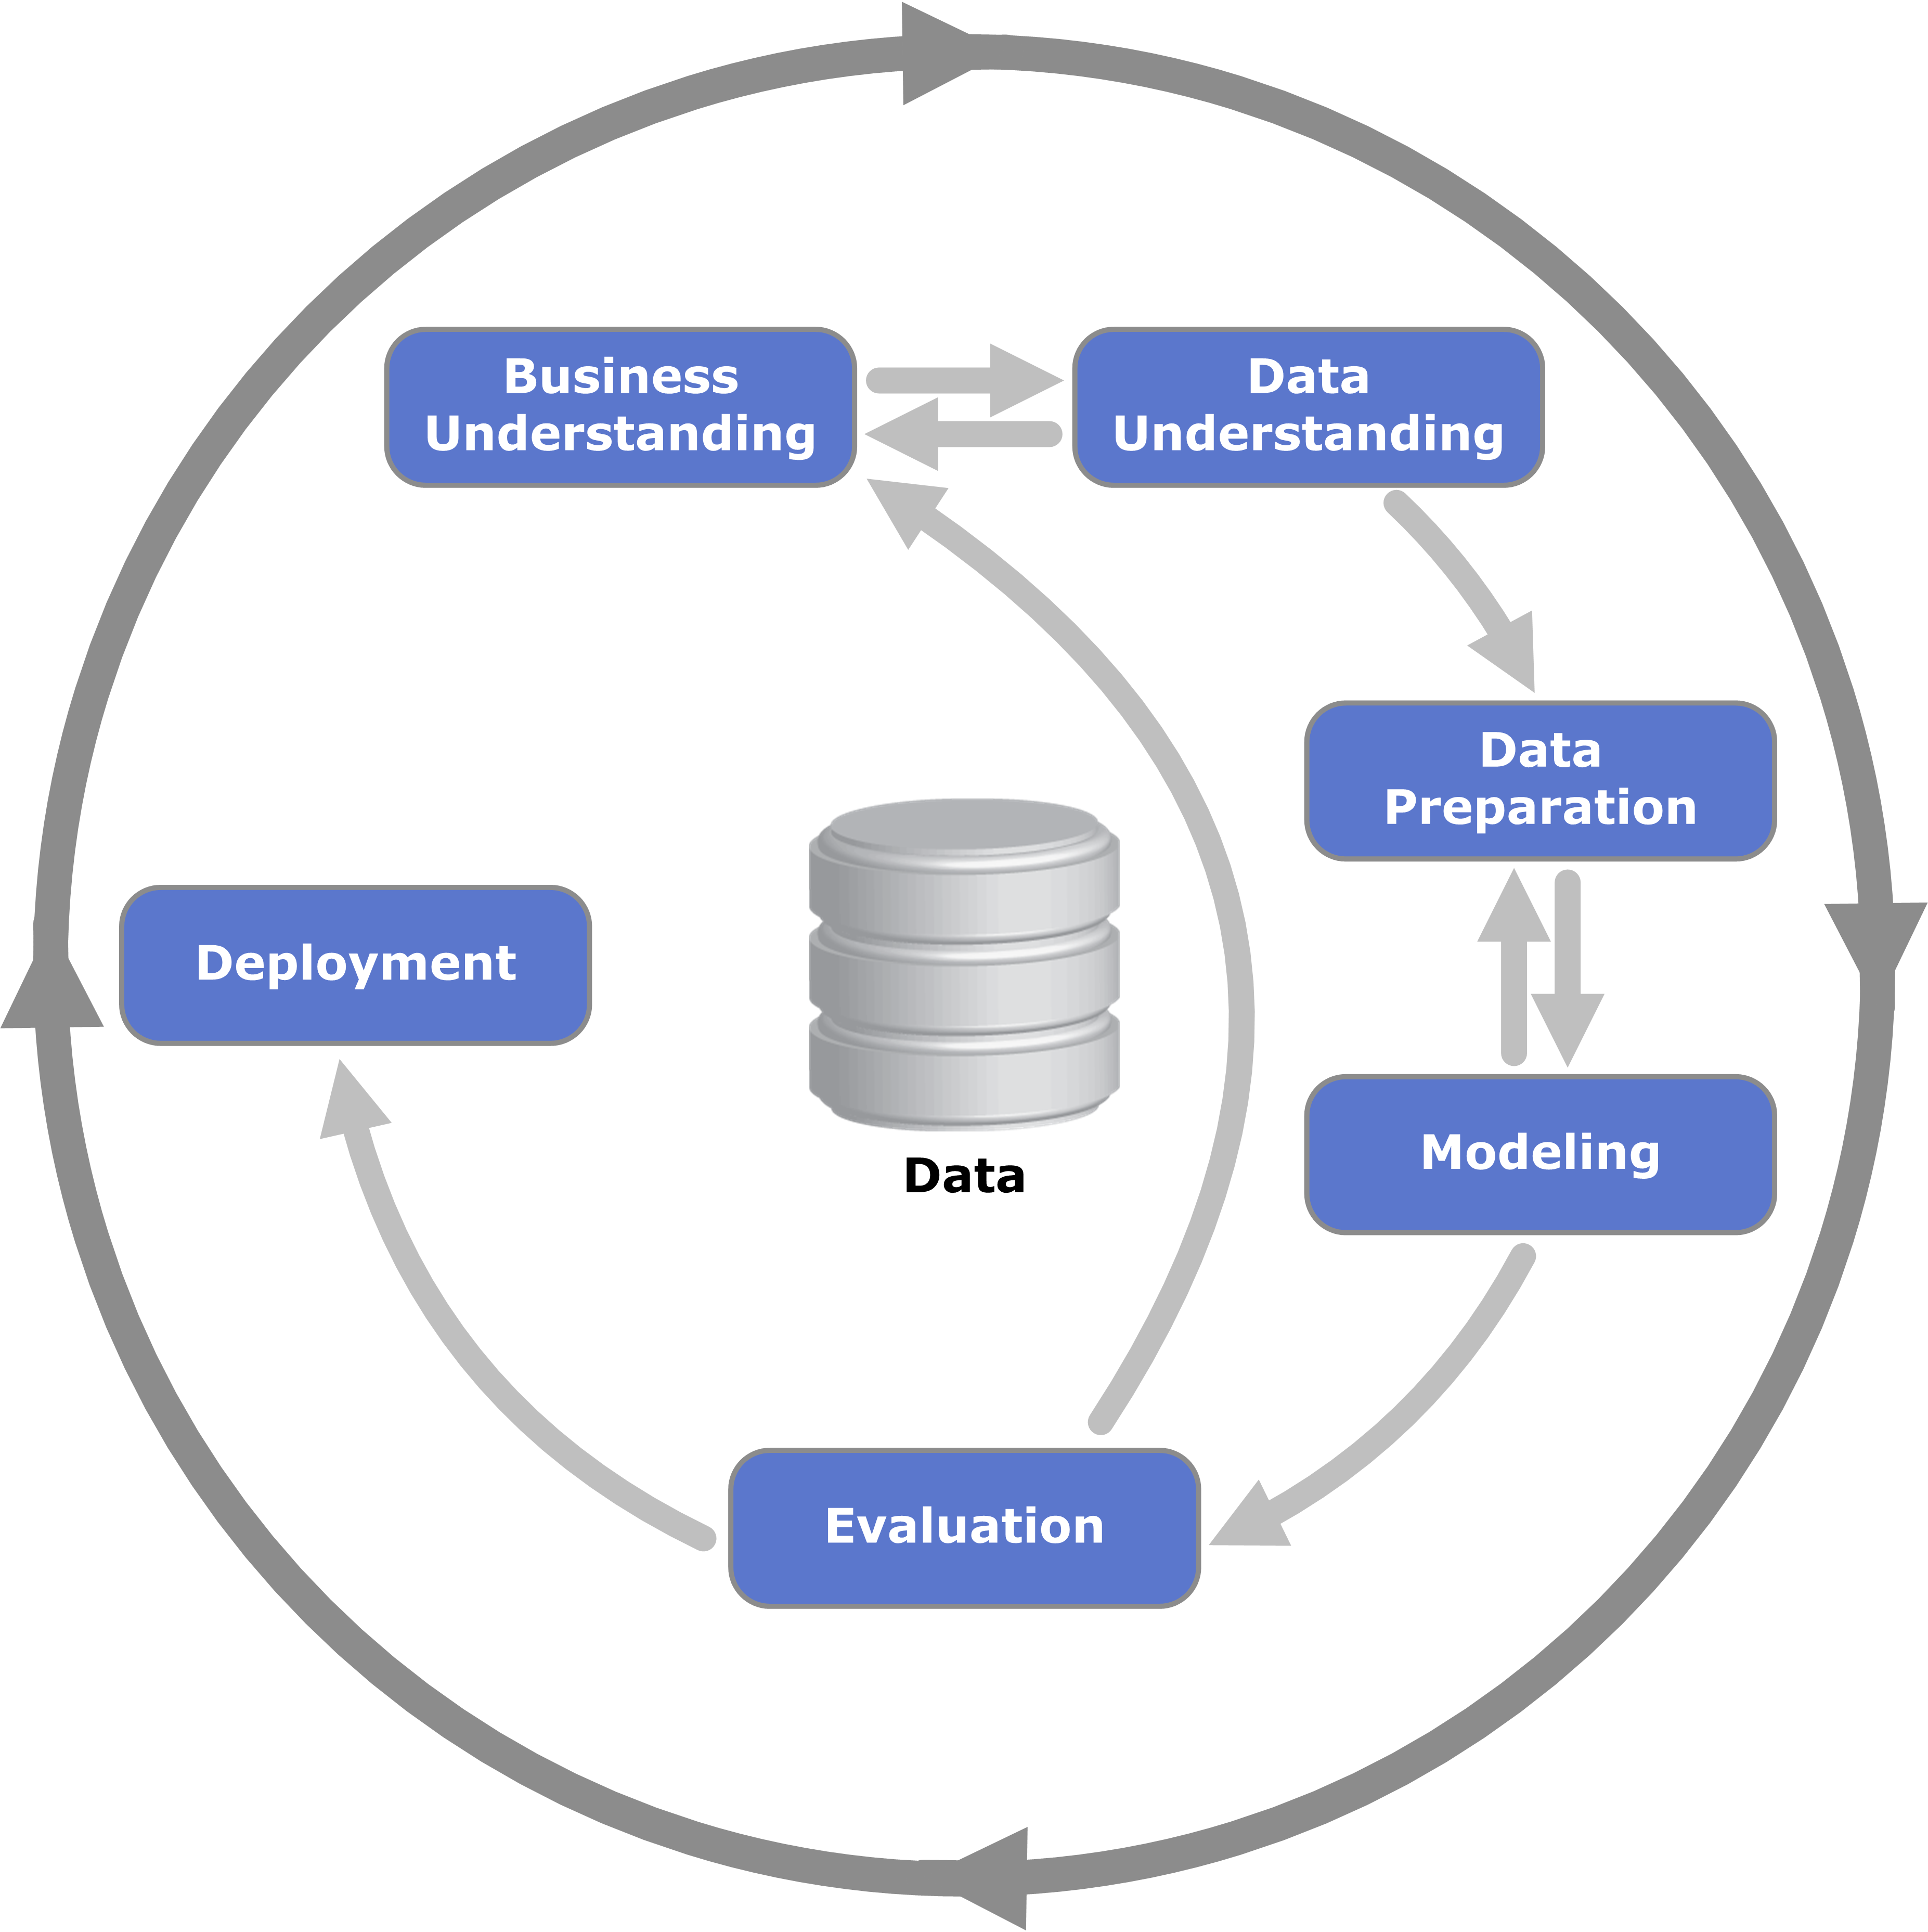
\includegraphics[width=0.5\linewidth,trim=0 0 0 0,clip]{crisp_dm.png}
    \caption{Phases of the CRISP-DM Reference Model, adapted from Shearer\cite{Shearer2000}.}
    \label{fig:crisp_dm}
\end{figure}

The first phase of CRISP-DM is business understanding, which involves such key elements as definition of project goals and their acceptance criteria and definition of the target variable of analysis\cite{Nisbet2018}.
Chapter~\ref{ch:background} focuses on definition of the goals of this thesis: it provides background information on land use and transportation models and some of the ongoing research efforts at UTTRI involving the housing market, outlines the role of Teranet's dataset in these efforts, challenges of its usage and the proposed solution.
Definition of the target variable is discussed in chapter~\ref{ch:ml_workflow} and criteria for model evaluation are discussed in chapter~\ref{ch:model_evaluation}.
Chapter~\ref{ch:spatial_and_temporal_relationships} covers the second phase of CRISP-DM process model, data understanding, and discusses the nature of spatial and temporal relationships of different data sources that are used in this master's thesis.
Chapter~\ref{ch:data_preparation} covers the third phase, data preparation, and presents the data preparation workflow designed to implement the relationships introduced in chapter~\ref{ch:spatial_and_temporal_relationships}.
Chapter~\ref{ch:ml_workflow} covers the fourth phase, modeling, and describes a prototype of a machine learning workflow to classify land use from the housing market dynamics.
Chapter~\ref{ch:model_evaluation} covers the fifth phase, evaluation, and presents the discussion of the results and chapter~\ref{ch:conclusion} presents the conclusion and outlines opportunities for future work.